\chapter{Introduction}

In this first chapter we want to familiarize the reader with the scientific
background of our work and its motivation. We hope to clarify what basic
questions the discipline of ultracold atom experiments tries to solve. In a
second part we want to elaborate on the concepts of localized optical
potential dynamcis and summarize the related work reported by the community.

Many body quantum systems studied inter alia in condensed matter physics are
experimentally challenging to access as quantum states have to be carefully
be prepared. As a way forward, experiments with ultracold atoms in optical
lattices give us a highly controllable environment where you can look at a
single atom level, prepare clean, well known states and reduce energy and time
scales to experimentally accessible quantities. Thus the platform of ultracold
atoms permit us to simulate and explore quantum effects and expand our current
understanding of quantum mechanics and statistical physics\cite{Gross2017}.
\begin{figure}[ht]
  \centering
  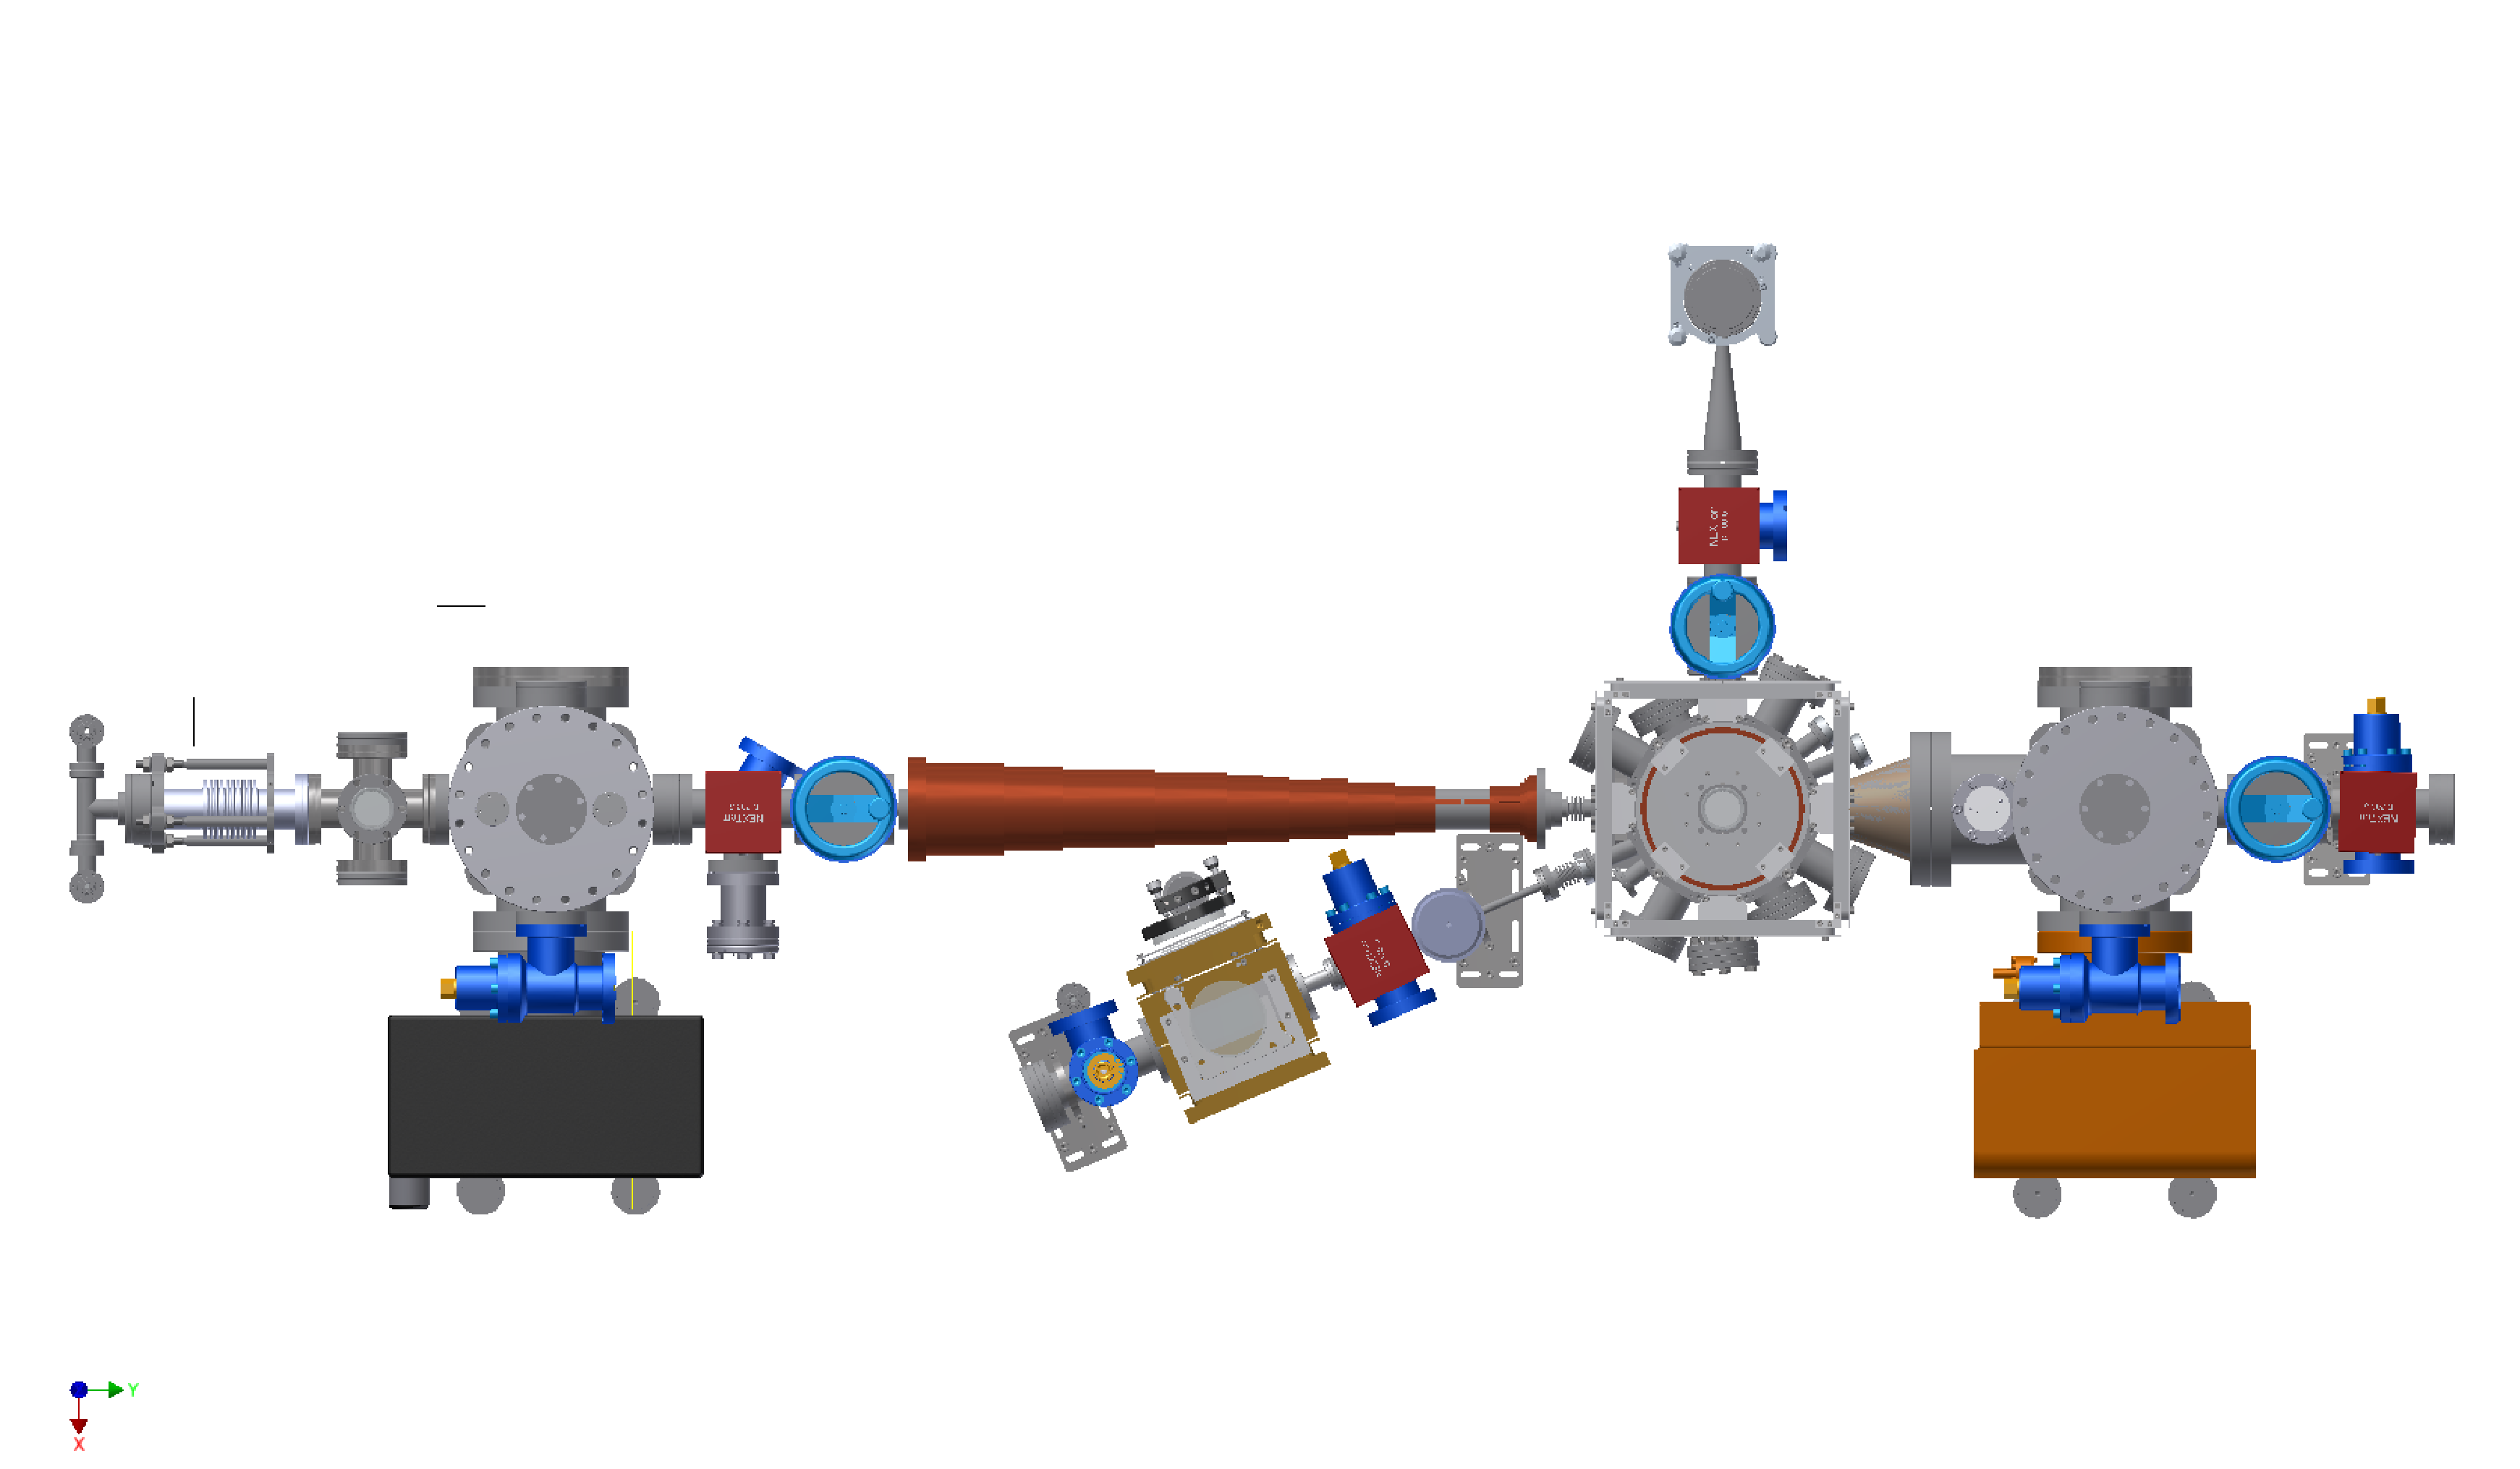
\includegraphics[width=\textwidth]{\figuredir{introduction/apparatus.pdf}}
  \captionsetup{width=.9\textwidth}
  \caption{Apparatus of the Cesium experiment. On the left-hand
    side an oven heats up a Cesium gas. A 2D \gls{mot} focuses the atoms as a
    particle beam twoards the pipe on the right. The Zeeman slower in the
    center of the apparatus creates a magnetic gradient such that the atoms
    are in resonance with the cooling laser antiparallel to their flight
    direction. In the 3D \gls{mot} atoms are cooled even further until they
    are finally loaded into the optical lattice inside the glass cell on the
    top where the actual experiments are conducted. Thank you to Till
    Klostermann and Hendrik v. Raven for providing the Cesium apparatus
    render.}\label{fig:ultracold_atoms_setup}
\end{figure}
The apparatus used for ultracold atoms experiments with optical lattices
comprises a vacuum system with multiple chambers and windows for optical
devices. \Cref{fig:ultracold_atoms_setup} depicts an exemplary apparatus used
for such an experiment with cesium atoms. The oven on the left-hand side heats
up an atom gas which will then travel to the right. Two orthogonal pairwise
windows are placed for transversal cooling and particle beam focusing in a 2D
\gls{mot}. The big tank to the right of the 2D \gls{mot} and the oven is used
for improving the vacuum and hosts a shutter to halt the particle beam. The
Zeeman slower in the center of the apparatus creates a magnetic field gradient
such that the atoms are always in resonance with the cooling laser
antiparallel to the momentum direction. Through this cooling step many of the
atoms can be captured in the 3D \gls{mot} where the atoms are cooled further.
Finally the atom cloud is transported to a glass cell at the top. The glass
cell is placed between two high numerical aperture objectives for in-situ,
single site imaging and addressing.

One major parameter to interact with the ultracold atom ensemble in the
experimental chamber is the optical lattice itself. In
\Cref{fig:optical_lattice} a cubic 2D optical lattice is presented.
\begin{figure}[ht]
  \centering
  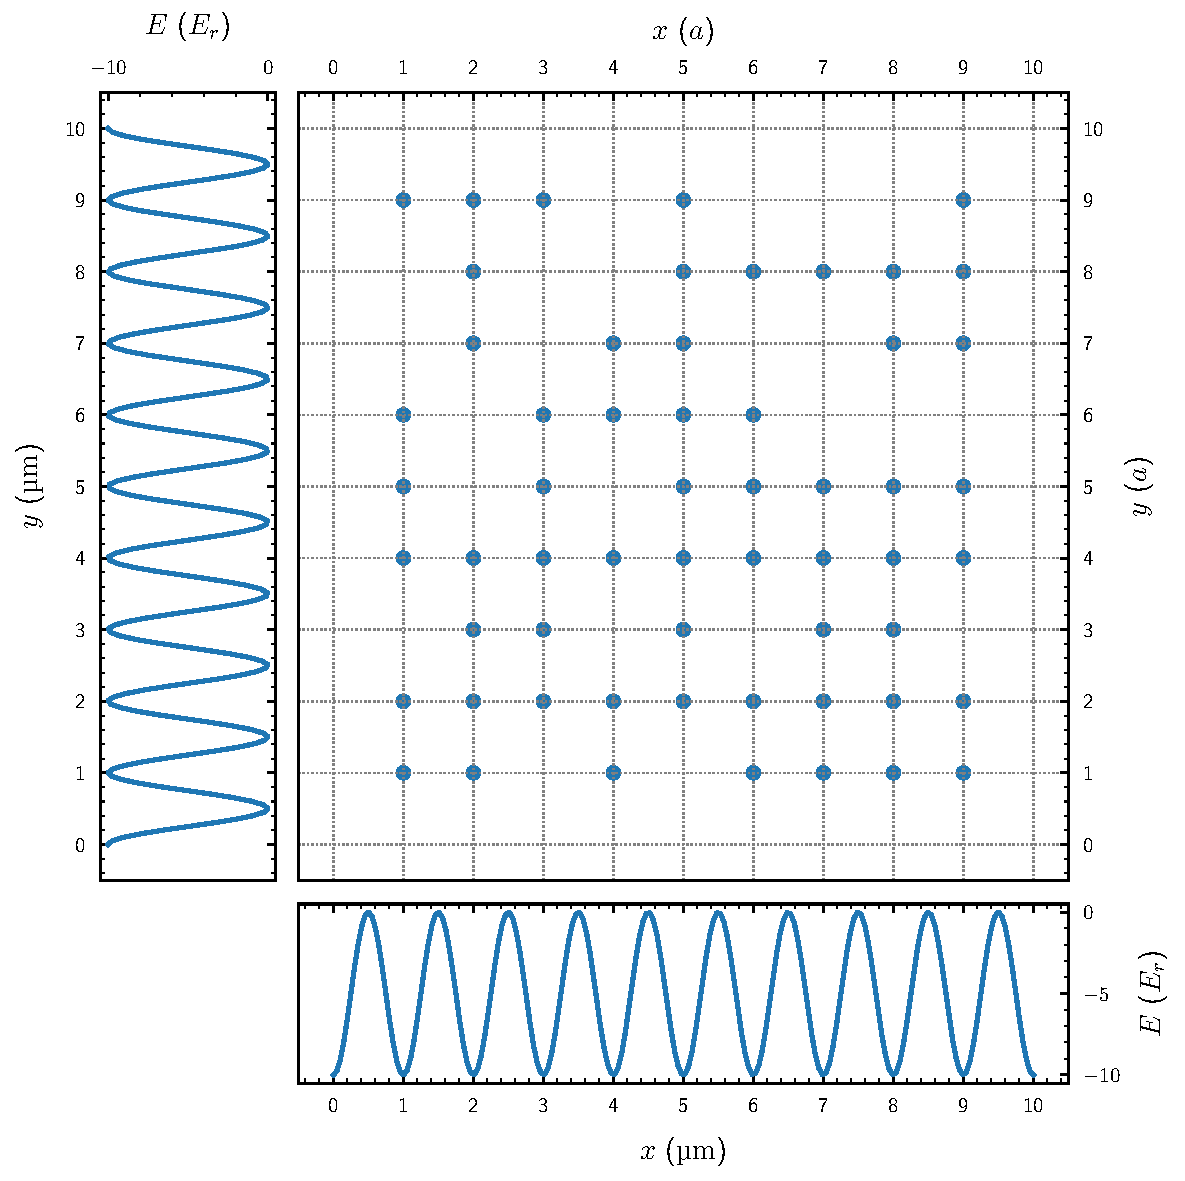
\includegraphics[width=.9\textwidth]{\figuredir{introduction/lattice-simple.pdf}}
  \captionsetup{width=.9\textwidth}
  \caption{Simple cubic 2D optical lattice optical lattice. The atoms (blue) sit on
    their respective lattice site created by the superposition of two
    periodic potentials.}\label{fig:optical_lattice}
\end{figure}
The atoms (blue) sit on their respective lattice sites (nodes in the gray
grid) which are created by the superposition of two optical potentials
(outer diagrams). In such periodic structures the atomic wave functions
already show amazing similarity to the electron wave functions known from
solid states physics but with much higher energies and longer time scales
because of the greater mass.
Though the simple cubic 2D optical lattice already offers many possiblities,
one can think of many more variations in terms of  lattice structure
inclduing hexagonal lattice structures or even lattices with lattice
substructure in the literature known as superlattices. Beside changes to the
global lattice structure we can also think of local changes to the lattice
structure. In \Cref{fig:optical_lattice_local_barrier} we have an embodiment
of a local optical lattice used to confine particles.
\begin{figure}[ht]
  \centering
  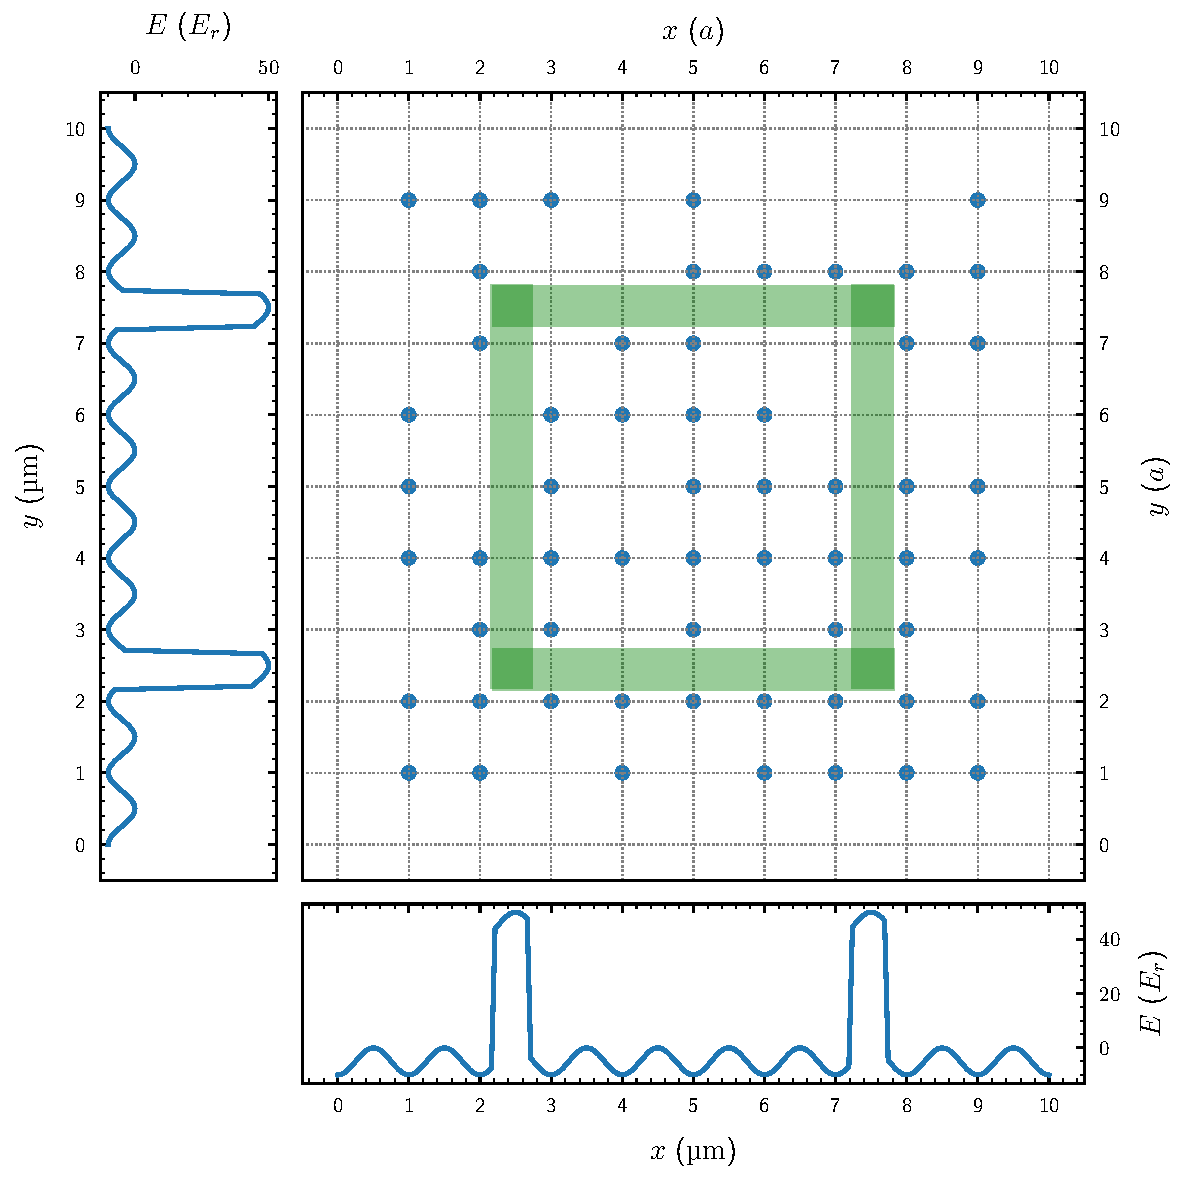
\includegraphics[width=.9\textwidth]{\figuredir{introduction/lattice-bar.pdf}}
  \captionsetup{width=.9\textwidth}
  \caption{Simple cubic 2D optical lattice with local barrier potential. The
    local barrier potential confines atoms inside the green box and limits
    interaction with the outer particles.}\label{fig:optical_lattice_local_barrier}
\end{figure}
By changing the barrier height one can control interaction with the the outer
particle ensemble which allows interesting constellations for thermodynamic
equilibrium processes.
In a second embodiment one can create a potential pot as illustrated in
\Cref{fig:optical_lattice_local_pot}.
\begin{figure}[ht]
  \centering
  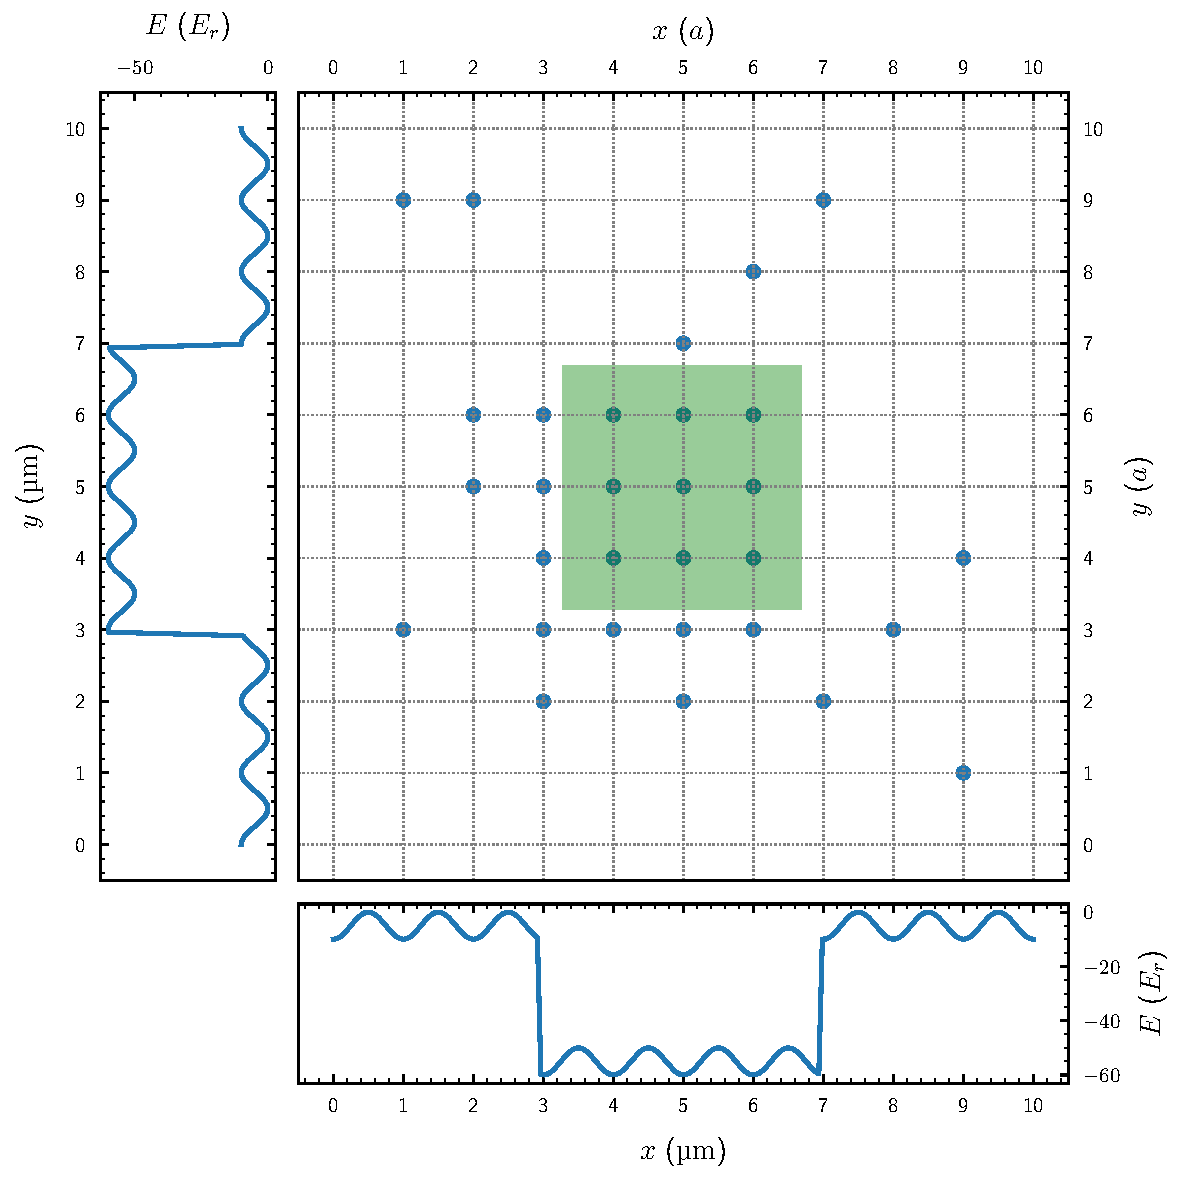
\includegraphics[width=.9\textwidth]{\figuredir{introduction/lattice-pot.pdf}}
  \captionsetup{width=.9\textwidth}
  \caption{Simple cubic 2D optical lattice with local pot potential. The local
    potental pot draws particles from the unperturbated lattice potential to
    an confined area.}\label{fig:optical_lattice_local_pot}
\end{figure}
Such a local potential pot would draw surrounding particles from the
unperturbated lattice potential and confine them. In an extreme case one could
also narrow the pot to only a single or a pair of atoms in order to simulate
lattice imperfections in solids.
Anyway there are of course many more possibilites to change the optical
lattice structure locally.

Local manipulations of atoms inside optical lattices have been known for some
time in the manifestatiion of optical tweezers that allow trapping, stacking
and sorting of particles\cite{Roxworthy2012}. Yet, only recently attempts to
interact with local particle clusters through high-precision time-averaged
optical potentials have been reported\cite{Roy2016}. The key concept to create
time-averaged local optical potentials is similar to the principle with what
cathode ray tube screens operate. The idea is to consecutively illuminate a
finite point set that covers the desired space. A complete passthrough of the
finite point set has to occur on a time scale short compared to the time scale
of the observed processes such that over average the passthrough yields an
effective potential in the observed process. In comparison to the state of the
art which uses mechanical mirror arrays for creation of local potentials
\cite{Roy2016} our approach exercises acousto-optical deflection by \gls{aod}.
In the following we continue on the ground work laid out in
\cite{Hertlein2017} which provided us with an optical setup for single-site
manipulation using \gls{aod} as well as the discussion of aperture limited
gaussian beam propagation.

We will start with the theoretical foundation of optical lattice potentials
and give more details on how the lattice potential alters under an additional
potential well. From there on we will estimate the required time scale set by
hopping frequency of atoms between lattice sites. After a short introduction
to direct digital signal synthesis we will calculate if and how the used
\gls{dds} met the previously found demands. That in place we can continue with
an overview of our experimental setup and results. The experiments separate in
a part concerning the radio electronics, a part dedicated to the intensity
transmission subject to the \gls{rf} signal and a final part where we attempt
to minimize the intensity transmission variance.
